\section{Durchführung}
\label{sec:Durchführung}
\begin{figure}[H]
  \centering
  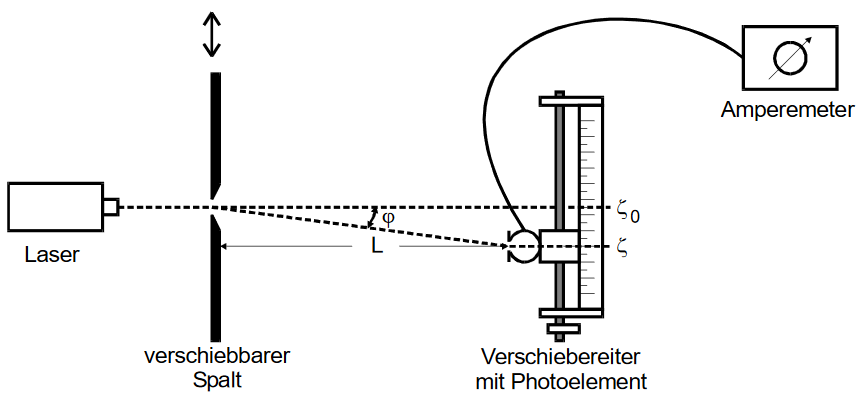
\includegraphics[height=5cm]{Aufbau.PNG}
  \caption{Versuchsaufbau zur Messung des Interferenzbildes \cite{sample}.}
  \label{fig:aufbau}
\end{figure}

Zur Untersuchung des Beugungsbildes des durch einen Laser ausgesendeten Lichtes wird
ein Versuchsaufbau entsprechend Abbildung \ref{fig:aufbau} verwendet.
Das Licht des Lasers trifft auf einen Einzel- bzw. Doppelspalt (je nach derzeitiger Messung).
Dort wird es dann gebeugt und verläuft hinter dem Spalt folglich in verschiedene Richtungen mit
unterschiedlicher Intensität. In einem Abstand groß zur Spaltbreite befindet sich dann ein verschiebbarer
Detektor (Photoelement). Dieser lässt sich senkrecht zur ursprünglichen Ausbreitungsrichtung des Lichtes
verschieben, sodass sich die Lichtintensitäten unter verschiedenen Beugungswinkeln messen lassen. Die
an dem Photoelement entstehenden Ströme können auf einem daran angeschlossenen Amperemeter abgelesen werden.

Auf diese Weise werden jeweils zwei Doppelspalte und ein Einzelspalt untersucht. Dabei wird jedoch für die
Doppelspalte lediglich die Intensitätsverteilung bis zum 2. Nebenmaximum und für den Einzelspalt bis zum 1.
Hauptmaximum gemessen.

Anschließend wird noch der Dunkelstrom bestimmt. Dazu wird die sich am Amperemeter einstellende Stromstärke
abgelesen, wenn kein Licht des Lasers auf das Photoelement trifft.
